\documentclass[10pt,twocolumn,letterpaper]{article}

\usepackage{ctex}
\usepackage{xeCJK}
\setCJKmainfont{SimSun}

\usepackage{cvpr}
\usepackage{times}
\usepackage{epsfig}
\usepackage{graphicx}
\usepackage{amsmath}
\usepackage{amssymb}

% Include other packages here, before hyperref.
\usepackage{xcolor}
\usepackage{subfigure}
\usepackage{multirow}
\usepackage{booktabs}
\usepackage{array}
\definecolor{purple}{rgb}{0.8,0,0.45}

% If you comment hyperref and then uncomment it, you should delete
% egpaper.aux before re-running latex.  (Or just hit 'q' on the first latex
% run, let it finish, and you should be clear).
\usepackage[pagebackref=true,breaklinks=true,letterpaper=true,colorlinks,bookmarks=false]{hyperref}

\cvprfinalcopy % *** Uncomment this line for the final submission

\def\cvprPaperID{****} % *** Enter the CVPR Paper ID here
\def\httilde{\mbox{\tt\raisebox{-.5ex}{\symbol{126}}}}

% Pages are numbered in submission mode, and unnumbered in camera-ready
\ifcvprfinal\pagestyle{empty}\fi
\begin{document}
	
	%%%%%%%%% TITLE
	\title{基于深度学习的自动文本摘要}
	
	\author{叶茂青,王珺,游小艳,徐嘉鸿,刘宇轩,李凌峰}
	
	\maketitle
	%\thispagestyle{empty}
	
	\begin{abstract}
		自动文本摘要指利用计算机程序自动地总结出文档的主要内容,自动文本摘要主要可分为抽取式摘要,即直接从原文中抽取一些句子组成摘要,和生成式摘要,即尝试理解原文的意思并生成出摘要,本文尝试使用不同的句向量生成方式和方法进行抽取式摘要,并对不同方法的效果和优缺点进行分析。
	\end{abstract}

	\section{句向量的生成}
	
	
	\subsection{词向量}
	Word2vec\cite{mikolov2013efficient},为一群用来产生词向量的相关模型。这些模型为浅层双层的神经网络,用来训练以重新建构语言学之词文本。网络以词表现,并且需猜测相邻位置的输入词,在word2vec中词袋模型假设下,词的顺序是不重要的。

训练完成之后,word2vec模型可用来映射每个词到一个向量,可用来表示词对词之间的关系。该向量为神经网络之隐藏层。

Word2vec依赖skip-grams或连续词袋(CBOW)来建立神经词嵌入。
	

	\subsection{句向量}
	一种简单的句向量生成就是通过拼接或者平均词向量的方式实现\cite{le2014distributed},但这种方式生成的句向量对于各个词的权重都是一致的,不符合语言的特性,相应的人们也提出了加权平均的方式,比如通过TF-IDF评估一个词语对于一个文档的重要程度,一个词语TF-IDF值与它在文档中出现频数成正比,与它在语料库中出现的频率成反比。TF-IDF由TF词频(Term Frequency)和IDF逆向文件频率(Inverse Document Frequency)相乘而得。
	但这种方式本质上无法理解上下文的语义,同一个词在不同的语境意思可能不一样,但是却会被表示成同样的句向量。也有人尝试用word2vec的方法进行扩展,使用与skip-grams类似的模型进行训练,如Skip-thought vectors\cite{kiros2015skip},但是这种方法过于直接,句子包含多种组合,通过一句话推知上下文不符合常识。因此目前效果更好的句向量生成方法通常采用有监督学习的方法,如InferSent\cite{conneau2017supervised},它使用Sentence Natural Language Inference(NLI)数据集(包含570k对标有3种类别的句子:中性,矛盾和包含)来在句子编码器之上训练分类器。 两个句子都使用相同的编码器进行编码,而分类器则是根据两个句嵌入构建的对表征进行训练。通过这种方法获取的句向量可以更有效的泛化到下游任务。而在2018年,语言模型开始向多任务训练转变,如BERT\cite{devlin2018bert},这可以让模型更充分的了解上下文的含义,生成更好的嵌入。
	
	\subsection{选取的方案}
	我们尝试采用了简单的平均和用TFIDF加权平均word2vec的方式获取的词向量,同时采取有监督学习获取句向量中比较经典的InferSent模型进行句向量的获取。


	\section{摘要生成}

	\subsection{生成式摘要}
	生成式摘要,即尝试理解原文的意思并生成出摘要,这种方式生成的摘要可以生成出原文不存在的句子,更贴近人类进行摘要的过程,也是目前热门的研究方向。利用深度学习解决生成式摘要最早的尝试在2015年,Rush等人\cite{rush2015neural}尝试用seq2seq模型生成文本摘要,2016年,Rush等人\cite{nallapati2016abstractive}又在原来的模型上做出改进,使用RNN网络代替了原来的FNN,并引入了Large Vocabulary Trick,Vocabulary expansion,Feature-rich Encoder,Switching Generator/Pointer等机制,提升了模型的表现。但此时的模型生成的摘要带有大量的UNK,可读性差,See等人\cite{see2017get}之后提出了将pointer-network\cite{vinyals2015pointer}引入进生成式摘要中,模型可以从原文中复制词汇,极大的改善了摘要的可读性。
	我们尝试使用pointer-generator networks\cite{see2017get}进行生成式摘要的训练,并复现了论文的结果,最后生成的部分摘要虽然可以与人工摘要不分上下,但大部分摘要都存在着语法问题,或是事实错误的问题。查找了更多文献后,我们并没有找到解决方案,且目前也没有良好的损失函数可以评判生成式摘要在语法,摘要准确度上的损失。考虑到训练时长(单Titan X需要3天的时间才能让网络收敛)和修改代码的难度,我们放弃了这一方案。

	\subsection{抽取式摘要}
	抽取式摘要从原文中抽取出一定句子作为摘要,由于是从原文中摘取的句子,这种方式生成的摘要不存在语法错误或事实错误的问题,但抽取的句子拼接在一起可能不通顺,将句子按原文的顺序排布一定程度上可以让摘要更加通顺,但是并没有从根本上解决这个问题。
	抽取式摘要的方式有很多,聚类,MMR,基于图排序的LexRank,Textrank,使用整数线性规划的ILP算法等,我们采用了聚类,MMR,Textrank这三种方法进行了尝试。
	
	\subsection{聚类}
	聚类算法是一种无监督学习的算法,给定一组数据点,可以用聚类算法将每个数据点分到特定的组中,假设我们从文本中抽取出三句摘要,通过句嵌入方法得到句子的嵌入后,我们可以使用聚类算法取得三个聚类中心,将其看作文章的三个信息点,计算每句话的嵌入与聚类中心的距离,对三个嵌入中心各选取一个距离最近的句子就可以得到摘取出的三句。

	\subsection{Textrank}
	Textrank算法基于著名的网页排序算法PageRank改动而来,PageRank算法的基本思想在于,一个页面如果被多个页面引用,说明该页面的重要性高,如果一个页面被重要性高的页面引用,相应的该页面的重要性也会提升。Textrank算法首先把所有文章整合成文本数据,接着把文本分割成单个句子,将句子转换成词向量从而构建节点连接图,用句子之间的余弦相似度作为边的权重并用矩阵存储起来,再将相似矩阵转换为以句子为节点、余弦相似度为边的图结构,计算句子的TextRank值,进而选出重要性高的N句作为摘要。


	\subsection{MMR}
	Maximal Marginal Relevance(MMR),不同于聚类方法和Textrank方法选取全文中最重要的句子,MMR算法可以均衡的考虑文章摘要的重要性和多样性,MMR算法的计算公式如下
	\begin{align}
	MMR\ Score(i) &= \lambda*score(i)-(1-\lambda)*max_{j} S(i,j) \\
	score(i) &= S(i,doc)
	\end{align}
	
	$\lambda$的值越大,代表得分更注重摘要的准确度,$\lambda$的值越小,代表得分更注重摘要的多样性。S函数计算文本与句子或句子与句子之间的相似度,相似度计算可以使用欧氏距离或者余弦相似度进行计算。
	
	\section{结果对比及分析}
	
	\subsection{评测指标}
	目前自动文本摘要的评测方法主要使用ROUGE\cite{lin2003automatic},ROUGE方法的基本思想是将模型生成的摘要与参考摘要两者的n-gram进行对比,从而计算召回率,准确率等数据,ROUGE的评价指标在自动文摘上主要使用ROUGE-N和ROUGE-L两个,ROUGE-N计算生成的摘要与标注摘要的n-gram召回率,通常用ROUGE-1/2来评估,ROUGE-L计算两个文本单元之间的最长公共序列。
	ROUGE评测方法作为一个2003年提出的方法,目前看来有很大的缺点,使用n-gram模型进行统计十分呆板,没有考虑到生成摘要在语法,事实等方面上的准确性,但目前来说还没有一个更好的评价方法可以取代ROUGE方法。
	以下的结果均使用python的rouge库进行计算,相比起论文中普遍使用的通过perl写的rouge评测工具,由于在语句处理上有差异,两者在得分上会有不同。

	\subsection{模型效果对比}
	\begin{table*}
	\setlength{\tabcolsep}{7mm}{
	\begin{tabular}{cccccc} \toprule
	Models  &  $ROUGE-1$  &  $ROUGE-2$  &  $ROUGE-L$    \\ \hline
	ORACLE                 & 56.61                       & 29.57                       & 38.48                       \\
	LEAD3                  & 40.62                       & 17.05                       & 24.86                       \\
	RANDOM                 & 29.15                       & 8.78                        & 17.62                       \\
平均词向量+聚类               & 31.47                       & 10.25                       & 18.89                       \\
TFIDF加权平均词向量+聚类        & 32.28                       & 10.85                       & 19.48                       \\
InferSent(Glove)+聚类    & 33.05                       & 11.42                       & 19.33                       \\
InferSent(FastText)+聚类 & 32.51                       & 11.03                       & 19.23                       \\
平均词向量+Textrank         & 31.39                       & 10.12                       & 18.18                       \\
InferSent+MMR          & 40.63                       & 17.06                       & 24.87    \\        
	\bottomrule
	\end{tabular}}
	\end{table*}

	ORACLE指从文章取出3句,在可能的组合中,ROUGE得分最大的组合,LEAD3选用文章的前三句,是常用且十分有效的Baseline,RANDOM采用随机选取3句的方式。
	InferSent模型有使用Glove进行嵌入的模型,也有使用FastText进行嵌入的模型,经过测试,使用Glove嵌入的模型在效果上更优,所以之后使用的InferSent都是使用Glove进行训练的模型。


	\subsection{结果分析}	
	经过我们的测试,TFIDF加权平均词向量一定程度上可以改善模型的表现,换用更好的句向量嵌入模型也可以让模型效果更好,而使用聚类方法和基于图的Textrank算法在表现上并没有太大差别。聚类中使用欧氏距离和余弦距离(代码中我们让向量归一化然后计算欧氏距离,两者在数学上是等价的)对模型的效果影响不大。
	聚类算法和Textrank算法表现不佳的原因一定程度上是因为这类算法只注重摘要的准确度而忽略了多样性。而MMR算法可以通过$\lambda$的值控制摘要在准确度和多样性之间的取舍,以下是我们使用不同的$\lambda$值做出的结果。
	\begin{center}\footnotesize
	\setlength{\tabcolsep}{1mm}{
	\begin{tabular}{cccccc} \toprule
	$lambda$  &  $ROUGE-1$  &  $ROUGE-2$  &  $ROUGE-L$    \\ \hline
	0.2                 & 22.05                       & 5.50                       & 13.58                       \\
	0.5                  & 40.63                       & 17.06                       & 24.87                      \\
	0.8                 & 31.44                       & 10.72                        & 16.99                       \\
       
	\bottomrule
	\end{tabular}}
	\end{center}

	在$\lambda$值偏大时,MMR算法更注重摘要的精确度,最后的ROUGE得分也与只注重摘要精确度的聚类算法和Textrank算法类似,而当$\lambda$值偏小时,模型偏向与摘要的多样性,模型的效果有明显的下降,当$\lambda$值选择恰当时,MMR算法的表现会明显优于聚类算法和Textrank算法。
	

	此外,在对聚类结果进行可视化的过程中,我们发现了聚类算法可能存在的问题,那就是文本中的极端数据可能会影响聚类的结果,下图是我们使用PCA降维后对聚类结果可视化的结果。可见由于文本中部分句子的嵌入有着严重的偏离,使用K-means聚类所得的聚类中心会向着这些样本偏移,从而造成选取的句子不属于文章的主要信息。虽然降维后的显示不能实际表示嵌入空间中各向量之间的位置,距离关系,但我们认为在高维空间上,这种问题仍然可能发生。我们考虑过使用其他的聚类算法进行尝试,但其他的聚类方法都难以直接套用在自动文摘任务上,如DBSCAN只会对样本分簇而不会给出聚类中心,无法评判句子的得分,Affinity propagation算法无法设定聚类数目,不能进行对比。
	\begin{figure}[h]
		\centering
		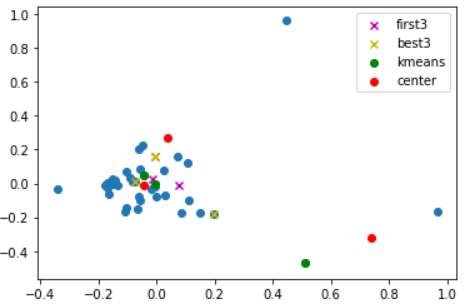
\includegraphics[width=\linewidth]{figures/1.png}
		\caption{聚类可视化}
	\end{figure}


	\section{总结}
	随着深度学习的发展,自动文本摘要的研究方向从抽取式摘要向生成式摘要转变,受限于时间和显卡性能,我们并没有使用生成式摘要的模型,而是尽可能的选用无监督学习的方式进行抽取式的摘要。从最后模型的结果不难看出,自动文本摘要要求对文章信息的精确把握,而这对嵌入模型和抽取模型都有着一定的要求,近年自动文本摘要的STOA模型也普遍使用了bert进行嵌入,利用深度学习建立良好的语言模型并不是易事,这是自动文本摘要受限的原因之一。
	
	自动文本摘要发展缓慢的另外一个原因,就是评测指标的问题,ROUGE提出这么久之后,依然没有一个更好的评价模型可以用于自动文本摘要领域,但今年也可以看到有研究人员开始重新思考自动文本摘要评价的指标,如Peyrard和Maxime为文本摘要提出了四个评价角度\cite{peyrard2019simple}。如果之后的研究可以设计出适合于自动文本摘要的目标函数,相信自动文本摘要领域会有更好的发展。
	

	
	{\small
		\bibliographystyle{ieee_fullname}
		\bibliography{egbib}
	}
	
	
\end{document}
